\section{Простые вычисления}

\subsection{Условие задания}
Выполнить задание. Номер варианта задает преподавателем. 

Проверить работу созданного приложения на приведенных тестовых примерах. Тесты сделаны на Visual Studio 2008, поэтому обращайте внимание только на первые шесть цифр после запятой.

Приложение должно содержать следующие компоненты:
\begin{enumerate}
    \item Заголовок формы должен отражать суть задания.
    \item Все элементы формы должны быть внятно подписаны (кнопки подписаны, у текстового поля должно быть написано, для чего оно нужно и т. д.)
    \item В коде должны быть комментарии и отступы (код должен быть легко читаем).
    \item Должна быть проверка ошибок - ввод не числа, ввод числа, находящегося за пределами ОДЗ, ввод числа, принадлежащего ОДЗ.
    \item Если надо ввести 2 значения, то в случае ввод букв в оба поля, ошибка должна быть у обоих полей; в случае ввода одной буквы - только у того поля, где буква.
\end{enumerate}

\textbf{Вариант 4.} Смотреть на рисунке \ref{task2_var4}.
\begin{figure}[H]
    \centering
    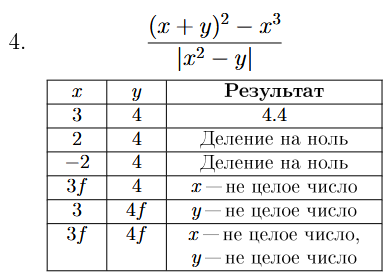
\includegraphics[width=0.5\linewidth]{lections/img/task2_var4.png}
    \caption{Задание 2 Вариант 4}
    \label{task2_var4}
\end{figure}

\subsection{Вид формы в конструкторе}
Создано окно приложения, содержащее три элемента TextBox, три элемента
Label, один элемент Button и один элемент ErrorProvider для обработки ошибок. Вид окна представлен на рисунке \ref{task2_form} \cite{никлаус2022алгоритмы}.
\begin{figure}[H]
    \centering
    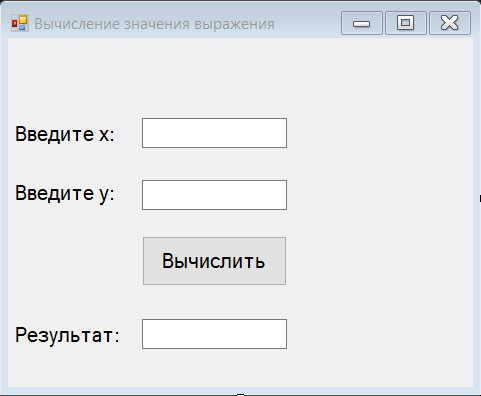
\includegraphics[width=0.5\linewidth]{lections/img/task2_form.png}
    \caption{Окно приложения «Вычисление значения выражения» открытое в конструкторе}
    \label{task2_form}
\end{figure}


\subsection{Таблица с описанием переименованных элементов формы}
Все измененные элементы формы указаны в таблице \ref{task2_attributes}.

\begin{table}[H]
\caption{Значения атрибутов элементов в приложении <<Вычисление значения выражения>>}
\begin{tabular}{|l|l|l|}
\hline
\textbf{\begin{tabular}[c]{@{}l@{}}Описание элементов\\ формы\end{tabular}} & \textbf{\begin{tabular}[c]{@{}l@{}}Список измененных\\ атрибутов\end{tabular}} & \textbf{\begin{tabular}[c]{@{}l@{}}Новое значение\\ атрибута\end{tabular}} \\ \hline
Форма MyForm                                                                & Text                                                                           & \begin{tabular}[c]{@{}l@{}}Вычисление значений\\ выражения\end{tabular}    \\ \hline
TextBox ввода x                                                             & Name                                                                           & x\_input                                                                   \\ \hline
TextBox ввода y                                                             & Name                                                                           & y\_input                                                                   \\ \hline
\begin{tabular}[c]{@{}l@{}}TextBox вывод\\ результата\end{tabular}          & Name                                                                           & output                                                                     \\ \hline
\multirow{2}{*}{Label у поля ввода x}                                       & Name                                                                           & x\_lbl                                                                     \\ \cline{2-3} 
                                                                            & Text                                                                           & Введите x:                                                                 \\ \hline
\multirow{2}{*}{Label у поля ввода y}                                       & Name                                                                           & y\_lbl                                                                     \\ \cline{2-3} 
                                                                            & Text                                                                           & Введите y:                                                                 \\ \hline
\multirow{2}{*}{Label у поля вывода}                                        & Name                                                                           & res\_lbl                                                                   \\ \cline{2-3} 
                                                                            & Text                                                                           & Результат                                                                  \\ \hline
\multirow{2}{*}{Кнопка "Вычислить"}                                         & Name                                                                           & solvebtn                                                                   \\ \cline{2-3} 
                                                                            & Text                                                                           & Вычислить                                                                  \\ \hline
\end{tabular}

\label{task2_attributes}
\end{table}


\subsection{Примеры правильной и неправильной работы}
После запуска программы на экране появляется окно на рисунке \ref{task2_launch1}.
\begin{figure}[H]
    \centering
    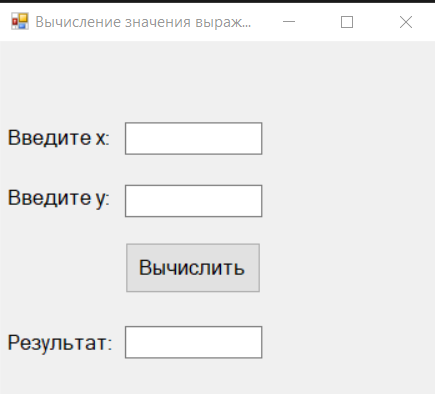
\includegraphics[width=0.4\linewidth]{lections/img/task2_launch1.png}
    \caption{Запуск программы}
    \label{task2_launch1}
\end{figure}
При вводе x и y в соответствующие поля и нажатии на кнопку "Вычислить" (на рисунке \ref{task2_launch2})
\begin{figure}[H]
    \centering
    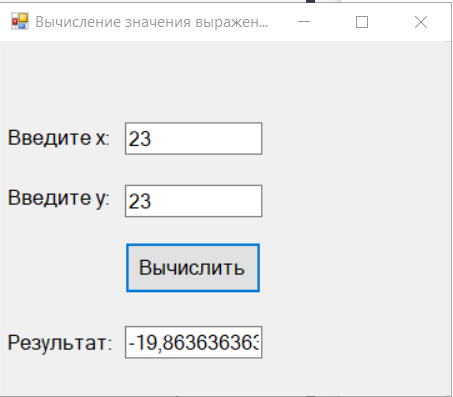
\includegraphics[width=0.4\linewidth]{lections/img/task2_launch2.png}
    \caption{Вычисление выражения}
    \label{task2_launch2}
\end{figure}
При попытке вычисления выражения такого, что $x^2 - y = 0$, вылезает ошибка <<деление на ноль>>  в поле вывода. (на рисунке \ref{task2_launch3}).
\begin{figure}[H]
    \centering
    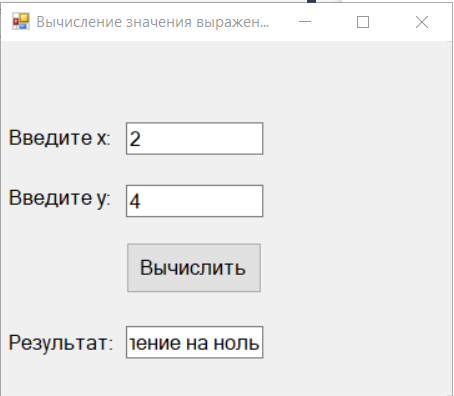
\includegraphics[width=0.4\linewidth]{lections/img/task2_launch3.png}
    \caption{Ошибка деления на ноль}
    \label{task2_launch3}
\end{figure}

\subsection{Примеры исходного кода}
Начало функции, выполняющейся при нажатии на кнопку <<Вычислить>>.
\begin{minted}[style=bw,
 linenos=true,
 breaklines=true,
 numbersep=5pt,
 tabsize=2,
 fontsize=\small,
 bgcolor=white]{cpp}
private: System::Void solvebtn_Click(System::Object^ sender, System::EventArgs^ e) {
	this->output->Text = ""; // Стираем поле вывода

	errors->SetError(x_input, String::Empty); // обнуляем ошибки
	errors->SetError(y_input, String::Empty);

	Int64 x, y; // Переменные для считывания полей ввода
	double result; // переменная для записи результата

	bool result_x = Int64::TryParse(this->x_input->Text, x); // записываем из полей ввода в соответствующие переменные
	bool result_y = Int64::TryParse(this->y_input->Text, y); // и проверяем на успешность выполнения парсинга

	if (!result_x) { // если неудачно
		errors->SetError(x_input, "Введено не целое число");
	}
	if (!result_y) {
		errors->SetError(y_input, "Введено не целое число");
	}
	if (result_x && result_y) { // если удачно
		if (x * x - y == 0) { // проверка на ОДЗ
			this->output->Text = "Деление на ноль";
		}
		else {
			result = (1.0) * ((x + y) * (x + y) - x * x * x) / (std::abs(x * x - y)); //Считаем
			this->output->Text = System::Convert::ToString(result); //Записываем результат
		}
	}
}
\end{minted}
Другие фрагменты кода расположены в приложении \ref{app:simple_calculations}.
\sectionbreak